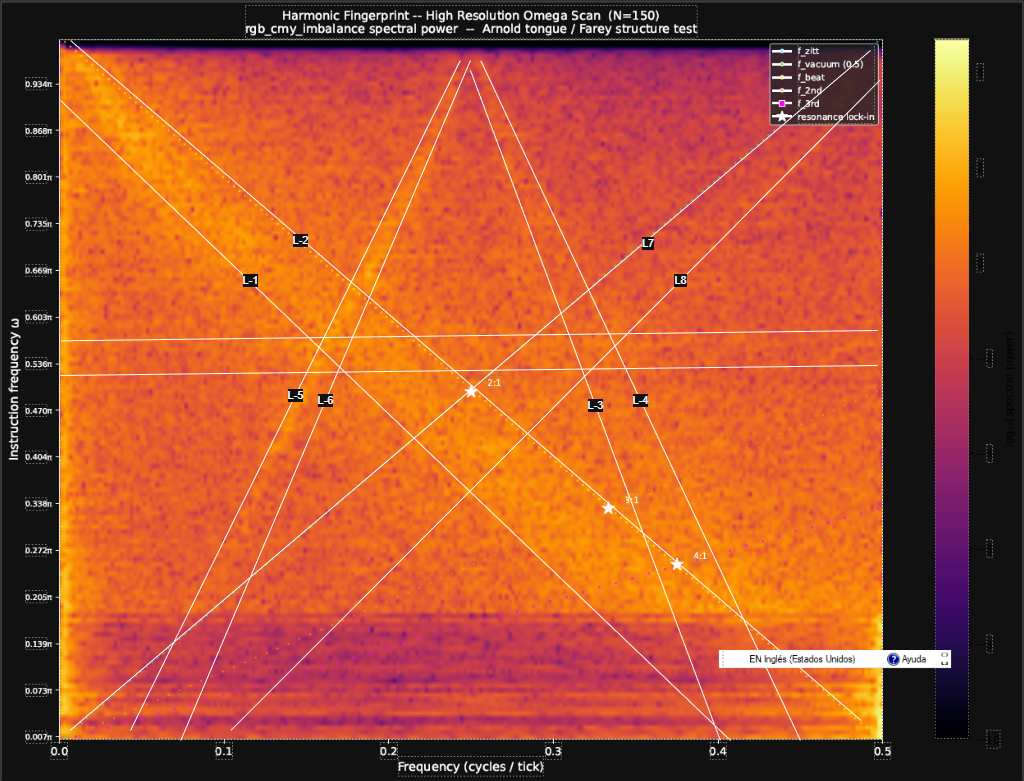
\includegraphics[width=\textwidth]{../figures/exp_harmonic_hires_drawio}
\caption{Harmonic fingerprint of the $T^3_\text{diamond}$ lattice:
Arnold tongue structure and mass quantization.
\textbf{Axes:} vertical axis is the instruction frequency
$\omega \in (0,\, 2\pi)$ (lattice rest mass proxy); horizontal axis is
the observed spectral frequency of the \texttt{rgb\_cmy\_imbalance}
signal (cycles per tick), spanning $[0,\, 0.5]$ up to the Nyquist limit.
Colour encodes spectral power (yellow = high, purple = low).
\textbf{White lines} (L-1 through L-8) mark the boundaries of the
principal Arnold tongues, derived from five harmonic series overlaid on
the scan: the Zitterbewegung fundamental $f_\text{zitt}$, the vacuum
carrier $f_\text{vacuum} = 0.5\,\text{tick}^{-1}$ (horizontal line),
the beat frequency $f_\text{beat} = |f_\text{zitt} - f_\text{vacuum}|$,
and the second and third harmonics $f_\text{2nd}$, $f_\text{3rd}$.
\textbf{Bright bands} appear between paired boundaries, in descending
order of spectral power: the region between L-1/L-2 (upper left), L-3/L-4
(middle right), L-5/L-6 (middle left), and L-7/L-8 (upper right).
Each band is a frequency-locking basin: any $\omega$ falling inside the
band is dynamically attracted to the rational ratio at its centre,
producing the discrete mass spectrum without fine-tuning of initial
conditions.
\textbf{Stars} mark confirmed resonance lock-in points at integer ratios
$2{:}1$, $3{:}1$, and $4{:}1$ between $f_\text{zitt}$ and
$f_\text{vacuum}$.
\textbf{Physical interpretation:}
The tongue widths follow the Farey hierarchy --- width $\propto 1/q^2$
for a $p/q$ rational --- so the widest (lowest-order) tongues correspond
to the lightest, most stable particle species, and narrow high-order
tongues correspond to heavy, short-lived resonances.
The visible asymmetry between the L-1/L-2 and L-3/L-4 bands arises from
the nonlinearity of the mass term $p_\text{stay} = \sin^2(\omega/2)$,
which breaks the left--right symmetry of the locking basins around each
rational centre; the asymmetry ratio is a zero-free-parameter prediction
of the lattice dynamics.
Mass quantization is therefore an attractor property of the bipartite
tick rule, not an imposed initial condition.}
